\section*{Auswertung}

Zur Auswertung wird die lange Messreihe für ein Teilchen als viele kurze \emph{random walks} betrachtet. Mit dem Ergodentheorem kann das Ergebnis gleichgesetzt werden mit der langen Messreihe.
Sämtliche Rechnungen sollen für $x$ und $y$ durchgeführt werden, im weiteren wird immer $x$ benutzt, aber die Auswertung für $y$ funktioniert analog.

\begin{enumerate}
\item Als erstes soll die Bewegung des Teilchens in einem $x$-$y$-Diagramm dargestellt werden. Hieran ist kurz zu erklären wie die Bewegung während der Messreihe verlief und welche Ergebnisse zu erwarten sind.

\item Sämtliche Messwerte müssen von Pixel in Meter umgerechnet werden. Dazu wird verwendet, dass zwischen zwei Skalenstrichen des Objektmikrometers $10\, \mu$m liegen.

\item Aus den Messdaten wird die Verschiebung $\Delta x$ zwischen zwei Bildern bestimmt. Für diese wird dann der Mittelwert und die Standardabweichung bestimmt. Was ist für den Mittelwert zu erwarten?

\item Die $\Delta x$ sollen in einem Histogram dargestellt und mit der Normalverteilung
\begin{equation}
  f(\Delta x, \mean{\Delta x}, \sigma) = \frac{1}{\sqrt{2 \pi \sigma^2}} e^{- \frac{(\Delta x - \mean{\Delta x})^2}{2 \sigma^2}}
\end{equation}
verglichen werden. Um die Skala anzupassen, muss die Normalverteilung mit der Anzahl der Messpunkte multipliziert werden.

\item Aus $\sigma(\Delta x)$ soll die Diffusionskonstante mithilfe von Gleichung (\ref{eq:diff}) berechnet werden. Die Zeit $t$ entspricht dem Zeitintervall zwischen zwei Bildern.

\item Die berechnete Diffusionskonstante kann dann in die Gleichung (\ref{eq:einstein}) eingesetzt werden um die Boltzmann-Konstante $k_B$ zu bestimmen. Diese ist mit dem Literaturwert zu vergleichen. Aus der Boltzmann-Konstante soll die Avogadro-Konstante $N_A$ bestimmt werden. Auch diese ist mit dem Literaturwert zu vergleichen.\\
Der Radius eines Polystyrol-Kügelchens beträgt $1\,\mu$m.
\end{enumerate}


\subsection*{Hinweise zur Auswertung}

\subsubsection*{Histogram und \emph{boxing-method}}
\begin{figure}[h!]
  \centering
  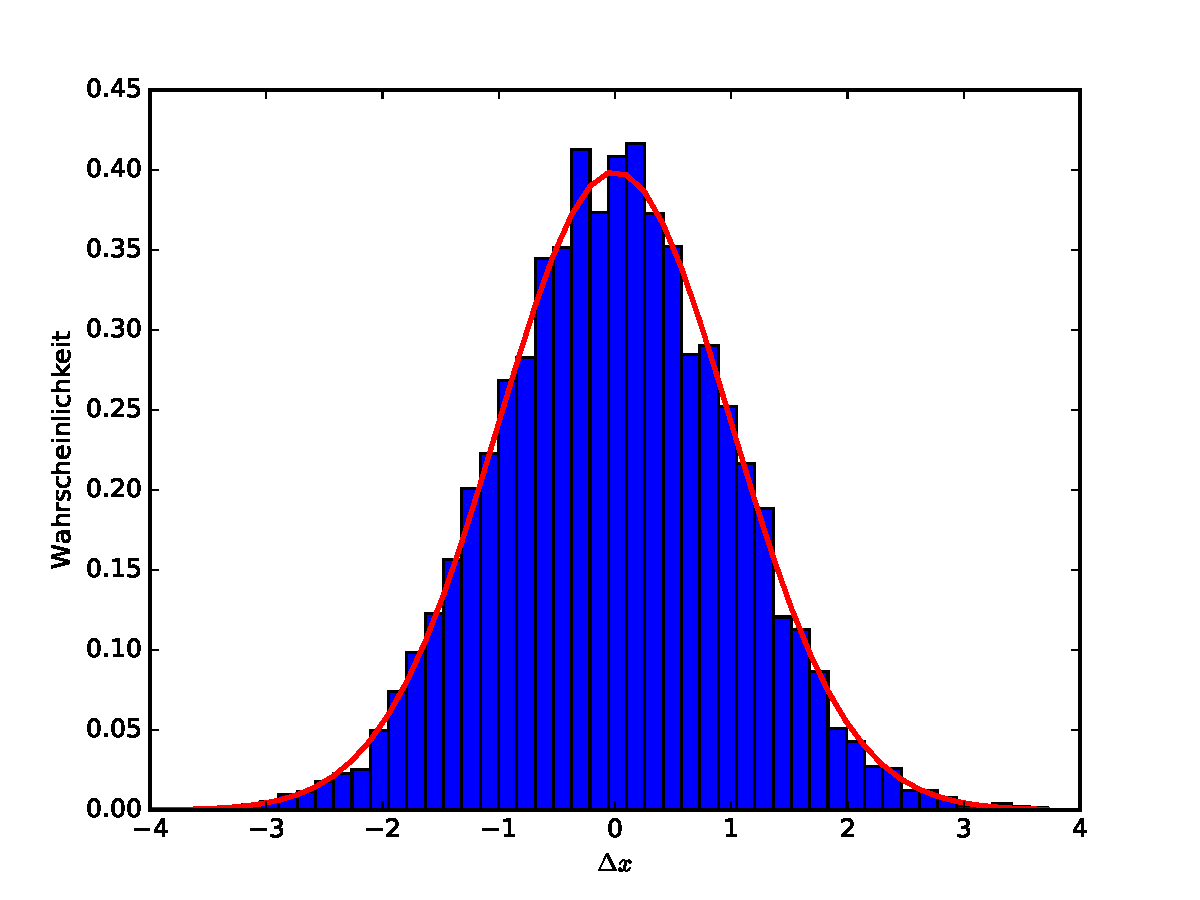
\includegraphics[width=0.7\textwidth]{figures/histogram}
  \caption{Histogram und zugehörige Normalverteilung}\label{fig:histo}
\end{figure}
Ein Histogram spiegelt die kontinuierliche Wahrscheinlichkeitsverteilung von diskreten Messdaten wieder. Anhand eines Histograms kann bestimmt werden, wie wahrscheinlich eine Messung innerhalb eines Intervals liegt. Darin besteht auch die größte Schwierigkeit dieser Methode: die geschickte Wahl der Intervalle. Alle Intervalle sollten die gleiche Größe haben, da sonst das Histogram verfälscht wird, aber die genaue Größe hängt von der untersuchten  Datenreihe ab.\\
Am einfachsten lassen sich die Intervalle finden, indem vorher über die Auflösung, also die Anzahl der Intervalle entschieden wird.  Ist die Auflösung zu fein, sind also die Intervalle sehr klein, dann ist in ihnen meist nur ein Messpunkt enthalten und die resultierende Verteilung ist nahezu eine Gleichverteilung. Ist sie hingegen zu grob, gibt es also zu wenig Intervalle, dann werden zu viele unterschiedliche Messwerte zusammengefasst. Um die Intervallgröße $\Delta$ zu bestimmen, kann die Formel
\begin{equation}
  \Delta = \frac{Max - Min}{\#Intervalle}
\end{equation}
benutzt werden. Dabei ist $Max$ der größte Messwert, $Min$ der kleinste Messwert und $\#Intervalle$ die Anzahl der Intervalle.\\
Danach wird die Anzahl der Messwerte in jedem Intervall gezählt und mit Balken aufgetragen, wie in Abbildung~\ref{fig:histo} zu sehen ist. Die Höhe der Balken liefert die Wahrscheinlichkeitsverteilung.

\subsubsection*{Histogramme mit SciDAVis}
Eine gute Grundlage für den Umgang mit SciDAVis, ``Auswertung von Messdaten'', kann bei den Unterlagen des Grundpraktikums gefunden werden.\\
Wenn die Messdaten eingelesen sind, müssen zuerst die Differenzen $\Delta x$ und $\Delta y$ bestimmt werden. Dazu muss jedes Element in einer Spalte von seinem Nachfolger abgezogen werden. Wenn der Name der Achse $x$ ist, dann können die $\Delta$ mit der Formel \verb|col("x", i) - col("x", i - 1)| berechnet werden. Vorsicht: Der erste Messwert muss aus der Betrachtung entfernt werden, da es keinen vorherigen Wert gibt um das $\Delta$ zu bestimmen.\\
Das Histogramm ist unter \emph{Diagramm $\rightarrow$ Statistische Diagramme $\rightarrow$ Histogramm} zu finden. SciDAVis setzt automatisch eine Intervallbreite, diese ist aber meistens nicht ideal. Um selber eine zu setzen kann, unter \emph{Format $\rightarrow$ Diagramm} das Histogramm ausgewählt werden. Unter \emph{Histogrammdaten} muss das Häkchen bei \emph{Automatische Einteilung} entfernt werden. Danach können bei \emph{Intervallbreite} eigene Werte eingesetzt werden.\\
Zuletzt fehlt noch ein Fit mit der Normalverteilung. Dieser geht sehr schnell, da SciDAVis eine eingebaute Funktion dafür hat. Diese liegt unter \emph{Analyse $\rightarrow$ Quick Fit $\rightarrow$ Gauss-Anpassung}. In dem \emph{Ergebnis-Log} lassen sich alle wichtigen Größen wiederfinden. Der Mittelwert ist $xc$ (Mitte) und die Standardabweichung $\sigma$ ist $w$ (Breite).
